\subsection{Bayesian logistic regression on MNIST}
\label{sec:mnist}

Bayesian logistic regression is applied to the handwritten digits $4$ and $9$ of the MNIST data set~\citep{lecun1998gradient}, shown in Figure~\ref{fig:mnist-data}, with the training set restricted to these digits. Each of the $n = 10{,}791$ training images, $5{,}342$ of the digit $4$ and $5{,}449$ of the digit $9$, is flattened, its pixel intensities are divided by $255$, and a constant $1$ is appended for the intercept, giving the vector $a_i \in \mathbb R^{785}$, with the label $y_i = 0$ for the digit $4$ and $y_i = 1$ for the digit $9$. With the prior $\mathcal N(0, \sigma_0^2 I_{785})$, $\sigma_0^2 = 10^{-3}$, the target is $\pi \propto e^{-U}$ on $\mathbb R^{785}$ with
\begin{equation}
    U(x) = \frac{|x|^2}{2\sigma_0^2} + \sum_{i=1}^{n} \Bigl( \log\bigl( 1 + e^{a_i \cdot x} \bigr) - y_i\, a_i \cdot x \Bigr) .
    \label{eq:mnist-potential}
\end{equation}
The stochastic gradient averages $P$ indices $\xi = (\xi_1, \dots, \xi_P)$, drawn independently and uniformly from $\{1, \dots, n\}$ at every step, independently of the Gaussian variables of the integrator:
\begin{equation}
    \nabla \hat U(x;\xi) = \frac{x}{\sigma_0^2} + \frac{n}{P} \sum_{p=1}^{P} \Bigl( \frac{1}{1 + e^{-a_{\xi_p} \cdot x}} - y_{\xi_p} \Bigr)\, a_{\xi_p} .
    \label{eq:mnist-minibatch-gradient}
\end{equation}

\begin{figure}[htb]
  \centering
  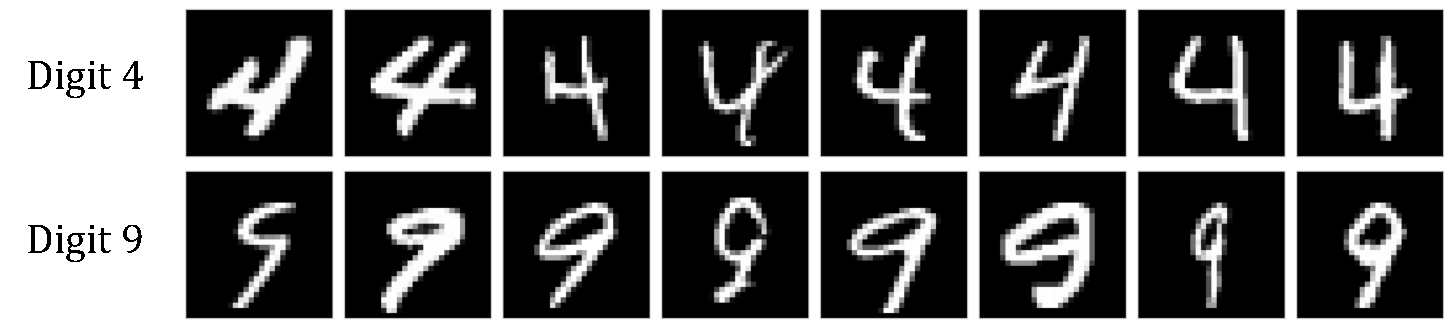
\includegraphics[width=0.72\textwidth]{figures/digit_illustration.pdf}
  \caption{Examples of the digits $4$ and $9$ of the MNIST data set.}
  \label{fig:mnist-data}
\end{figure}

The test functions measure the posterior in directions of different curvature. Let $x_*$ be the minimizer of $U$, computed by L-BFGS with the full gradient, and let $\lambda_1 \Ge \dots \Ge \lambda_8$ be the $8$ largest eigenvalues of $\nabla^2 U(x_*)$, with orthonormal eigenvectors $v_1, \dots, v_8$. In the standardized coordinates
\begin{equation}
    z_j(x) = \sqrt{\lambda_j}\, v_j \cdot (x - x_*) , \qquad j = 1, \dots, 8 ,
    \label{eq:mnist-local-coordinates}
\end{equation}
the $16$ bounded test functions are
\begin{align}
    f_{C_j}(x) &= \cos z_j(x) , && j = 1, \dots, 8 ,
    \label{eq:mnist-cosine-observables} \\
    f_{G_j}(x) &= e^{-z_j(x)^2/2} , && j = 1, \dots, 4 ,
    \label{eq:mnist-gaussian-1d-observables} \\
    f_{G_{j,k}}(x) &= e^{-(z_j(x)^2 + z_k(x)^2)/2} , && (j,k) \in \{(1,2), (3,4), (5,6), (7,8)\} .
    \label{eq:mnist-gaussian-2d-observables}
\end{align}
The cosines $f_{C_j}$ probe single directions, and the Gaussians $f_{G_j}$ and $f_{G_{j,k}}$ the concentration near $x_*$ in $1$ or $2$ coordinates.


The step size follows \citet[Section~4]{brosse2018promises} for logistic regression with the Gaussian prior, $h = (\sigma_0^{-2} + \delta/4)^{-1} \approx 8.5099 \times 10^{-6}$, where $\delta$ is the largest eigenvalue of $\sum_{i=1}^n a_i \otimes a_i$. For each batch size $P = 1024, 2048, 4096$, SGLD and SGLM are run in $20$ pairs of trajectories, the $2$ trajectories of a pair using the same indices $\xi$ and the same Gaussian variables. Every trajectory starts at $x_*$, discards its first $2^{14}$ steps and retains the next $2^{17}$ states. The reference values $\widehat\pi_{\mathrm{ref}}(f)$ are the pooled averages of $4$ independent chains of NUTS~\citep{hoffman2014no} with the full gradient, which leaves $\pi$ invariant, each with $2^{19}$ retained states after $2^{14}$ adaptation steps. The chains use the implementation of NUTS in Pyro~\citep{bingham2019pyro}, in the coordinates whitened by the Cholesky factor of $\nabla^2 U(x_*)$, with the target acceptance rate $0.9$, the maximal tree depth $10$, and the step size and a diagonal mass matrix adapted during the adaptation steps. The $4$ chains agree closely for all $16$ test functions, their Monte Carlo errors are small compared with the errors below, and these Monte Carlo errors are included in the resampling intervals below.

For each integrator, batch size and test function $f$, the estimates use the first $N$ retained states, for every multiple $N$ of $8192$ up to $2^{17}$. With $Z_{r,k}$ the $k$th retained state of the repetition $r = 1, \dots, 20$, let
\[
  \widehat\mu_r=\frac{1}{N}\sum_{k=0}^{N-1}f(Z_{r,k}),
  \qquad
  \overline\mu=\frac{1}{20}\sum_{r=1}^{20}\widehat\mu_r
\]
be the time average and its mean over the repetitions. The estimated finite-time bias and the variance of the time averages are
\[
  \widehat b=\overline\mu-\widehat\pi_{\mathrm{ref}}(f),
  \qquad
  \widehat V=\frac{1}{20}\sum_{r=1}^{20}
    (\widehat\mu_r-\overline\mu)^2.
\]
The reported estimate of the MSE \eqref{eq: mse} is
\begin{equation}
  \widehat{\MSE}_f(N,h)
  =\frac{1}{20}\sum_{r=1}^{20}
   \bigl(\widehat\mu_r-\widehat\pi_{\mathrm{ref}}(f)\bigr)^2
  =\widehat V+\widehat b^{\,2}.
  \label{eq:mnist-mse}
\end{equation}
The variance is that of the time averages over the repetitions, not of single states, and the bias is that of time averages of finite length, not the numerical bias of the invariant distribution.


\begin{figure}[htb]
  \centering
  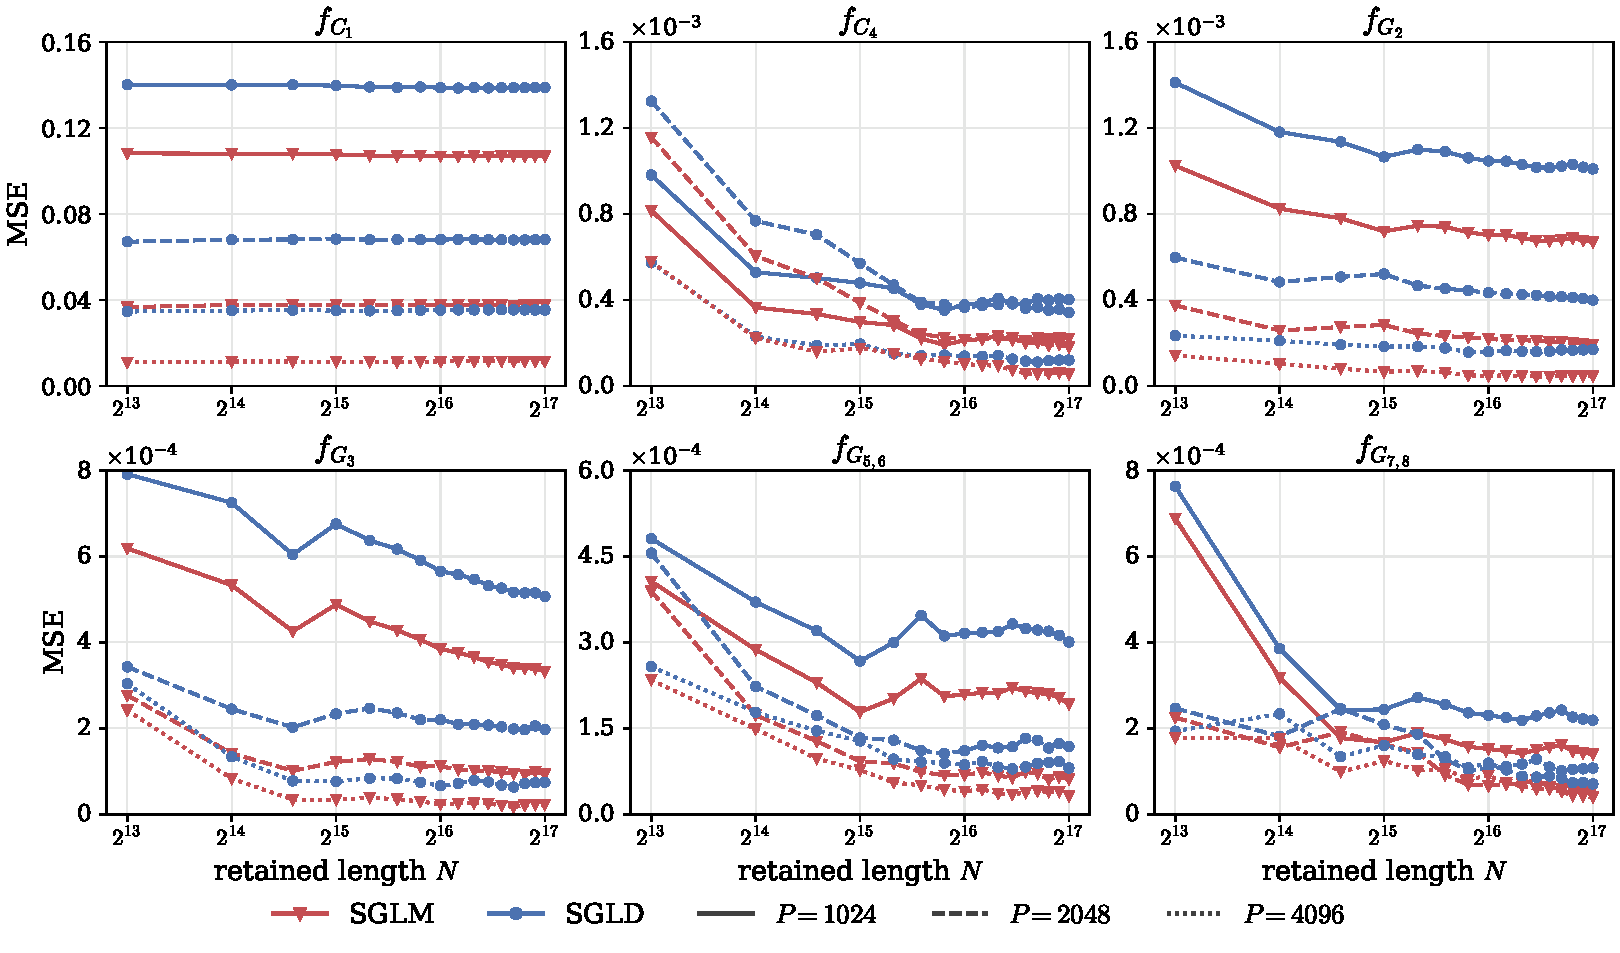
\includegraphics[width=\textwidth]{figures/mnist_mse.pdf}
  \caption{Estimated MSE \eqref{eq:mnist-mse} of the time averages of SGLD and SGLM for $f_{C_1}, f_{C_4}, f_{G_2}, f_{G_3}, f_{G_{5,6}}$ and $f_{G_{7,8}}$ against the retained length $N$, with $20$ pairs of trajectories for each batch size $P$.}
  \label{fig:mnist-mse}
\end{figure}

Figure~\ref{fig:mnist-mse} shows $2$ test functions of each form, $f_{C_1}, f_{C_4}, f_{G_2}, f_{G_3}, f_{G_{5,6}}$ and $f_{G_{7,8}}$, which together involve all $8$ coordinates \eqref{eq:mnist-local-coordinates}. For $f_{C_1}$ the estimated MSE is nearly constant in $N$, so longer averages bring little improvement in the tested range. For $f_{C_4}$ and $f_{G_{7,8}}$, several curves decrease markedly at small $N$ and then level off. For $f_{G_2}$, $f_{G_3}$ and $f_{G_{5,6}}$, longer averages are particularly beneficial for SGLM at $P = 4096$, whose errors fall below those of SGLD. The leveling off of several curves indicates a part of the error from the numerical bias, which longer averages at fixed $h$ and $P$ cannot remove.

At the largest retained length $N = 2^{17}$, SGLM has the smaller estimated MSE for all $16$ test functions at each of the $3$ batch sizes, that is, in all $48$ comparisons, and in each of them the $95\%$ interval of $\widehat{\MSE}_{\mathrm{SGLD}} - \widehat{\MSE}_{\mathrm{SGLM}}$ obtained by resampling the $20$ pairs with replacement lies above $0$. For each test function and batch size, the comparison at $N = 2^{17}$ uses the quantities
\begin{gather*}
    \text{MSE Reduction} = 100 \biggl( 1 - \frac{\widehat{\MSE}_{\mathrm{SGLM}}}{\widehat{\MSE}_{\mathrm{SGLD}}} \biggr) \% , \\
    \text{Bias Ratio} = \frac{|\widehat b_{\mathrm{SGLM}}|}{|\widehat b_{\mathrm{SGLD}}|} , \qquad
    \text{Variance Ratio} = \frac{\widehat V_{\mathrm{SGLM}}}{\widehat V_{\mathrm{SGLD}}} .
\end{gather*}
A positive MSE reduction and ratios below $1$ favor SGLM. Table~\ref{tab:mnist-endpoint} gives the median of each quantity over the $16$ test functions.

\begin{table}[htb]
	\centering
	\small
	\begin{tabular}{cccc}
		\toprule
		$P$ & MSE Reduction & Bias Ratio & Variance Ratio \\
		\midrule
		1024 & 34.6\% & 0.784 & 1.020 \\
		2048 & 46.5\% & 0.677 & 1.018 \\
		4096 & 63.3\% & 0.516 & 1.032 \\
		\bottomrule
	\end{tabular}
	\caption{Comparison of SGLM with SGLD at $N = 2^{17}$: the median over the $16$ test functions of each quantity, computed for each test function.}
	\label{tab:mnist-endpoint}
\end{table}

The median MSE reduction grows with the batch size, from $34.6\%$ to $63.3\%$, while the median variance ratio stays close to $1$ and the median bias ratio decreases from $0.784$ to $0.516$: the gain of SGLM comes from smaller finite-time biases, not from smaller fluctuations. This trend in $P$ is consistent with the separation of the errors in Theorem~\ref{thm: sglm mse}: a batch of $P$ independent stochastic gradients reduces the contribution of the gradient noise to $\Sigma^2 h^2 / P^2$, while the discretization error contributes $h^4$ for SGLM and $h^2$ for SGLD in \eqref{eq: sgld mse}. In the bias, the coefficient \eqref{eq: bias coefficient} of SGLM is divided by $P$, while the coefficient \eqref{eq: sgld coefficient} of SGLD keeps the contribution of the discretization error of EM at every batch size.